\documentclass[a4paper, 11pt]{report}
\usepackage[T1]{fontenc}
\usepackage{lmodern}
\usepackage[polish]{babel}
\usepackage[utf8]{inputenc}
\usepackage{enumerate}
\usepackage{multirow}
\usepackage{graphicx}
\usepackage{caption}
\usepackage{subcaption}
\usepackage{listings}
\usepackage{fancyhdr}
\usepackage{tikz}
\usepackage{latexsym}
\usepackage{subfig}
\usepackage{color}
\usepackage{pdflscape}
\pagestyle{fancy}
\usepackage[all,cmtip]{xy}
\selectlanguage{polish}
\title{\huge{Praca magisterska\\ ,,Bezprzewodowy system sterowania z wykorzystaniem systemu czasu rzeczywistego FreeRTOS''}}
\author{Jan Głos}
\date{26.06.2018}
\lhead{Praca magisterska} 																																						% określa lewą część nagłówka
\chead{} 																																															% określa środkową część nagłówka
\rhead{,,Bezprzewodowy system sterowania z wykorzystaniem systemu czasu rzeczywistego FreeRTOS''} 		% określa prawą część nagłówka
\lfoot{} 																																															% określa lewą część stopki
\cfoot{\thepage} 																																											% określa środkową część stopki
\rfoot{} 																																															% określa prawą część stopki
\newcommand{\ods}{\hspace*{1em}}

% ***@ DOCUMENT BEGIN @***

\begin{document}
\thispagestyle{empty}
\begin{figure}[t]
\centering

\includegraphics[width=14cm]{files/pk}
\end{figure}
\vspace{8cm}
\begin{Huge}
\begin{center}
\textsc{Wydział Inżynierii \\*Elektrycznej i Komputerowej}
\end{center}
\end{Huge}
\vspace{2cm}
\begin{center}
\begin{huge}
Praca magisterska\\ ,,Bezprzewodowy system sterowania z wykorzystaniem systemu czasu rzeczywistego FreeRTOS''\\
\end{huge}
\vspace{2cm}
\begin{LARGE}
Jan Głos\\

\vspace{5cm}
Promotor: \hfill Dr inż. Wojciech Mysiński
\hfill
\end{LARGE}
\end{center}

\newpage
\begin{small}
\tableofcontents
\end{small}


\newpage
\chapter{Wprowadzenie}
\section{Cel pracy}

Celem pracy jest projekt oraz realizacja sterownika, pracującego w systemie automatyki budynkowej KNX. Sterownik powinien współpracować ze wszystkimi dostępnymi urządzeniami\footnote{Mowa o urządzeniach z licencją organizacji Konnex}, zgromadzonymi w ramach jednej sieci KNX. Urządzenie musi więc pracować w standardzie, umożliwiającym komunikację z danymi aparatami za pośrednictwem wspólnej magistrali.
\\ \\
Głównym zadaniem jest więc zbudowanie platformy opartej na \\mikrokontrolerze, która w zależności od potrzeb może zostać zaprogramowana do różnych zadań. Środowisko takie powinno zapewniać szereg funkcji, użytecznych na stanowisku laboratoryjnym. Różnorodność zastosowań, nie może być zbyt mocno ograniczona przez sprzęt, zdecydowano się zastosować nowoczesny mikrokontroler o dużej ilości peryferiów i odpowiedniej mocy obliczeniowej. Platforma może zostać więc wykorzystana do sterowania oprawami świetlnymi\footnote{Pracującymi oczywiście w omawianym standardzie}, urządzeniami klimatyzacyjno-grzewczymi\footnote{ang. HVAC - Heating, Ventilation, Air conditioning} oraz roletami. Może także zostać skonfigurowana by pracować jako urządzenie wykonawcze np. moduł załączający oprawy oświetleniowe. \\Rola urządzenia w systemie KNX może zatem być różna i zależy od decyzji programisty.
Platforma może być przeznaczona jako aparat dydaktyczny, umożliwia pracę z systemem KNX oraz samym systemem\\ mikroprocesorowym.

%%

\newpage
\ods Głównym celem (i jednocześnie największą zaletą) stosowania systemów automatyki budynkowej w domach jednorodzinnych oraz budyknach usługowych, jest oszczędność. Jednak koszty, jakie ponosi inwestor na etapie projektowania i montażu systemu automatyki budynkowej, są wielokrotnie wyższe, niż koszty klasycznej instalacji elektrycznej, co najczęściej zniechęca do takiej inwestycji. Natomiast dedukcja zorientowana przyszłościowo, musi wziąć pod uwagę także koszty późniejszej eksploatacji budynku. \\Automatyczne sterowanie urządzeniami HVAC, oprawami świetlnymi czy nawet roletami, pozwala zmniejszyć wydatki. Producenci sprzętu 'smart home' oraz entuzjaści tego typu rozwiązań, zwracają uwagę: \\
\begin{quote}
	,,ZZZ\% \footnote{,,zzz'', www.Zzz.pl}
\end{quote}

%NEW PAGE
\newpage
\chapter{Część teoretyczna}
\section{Systemy otwarte}
\ods KNX/EIB jest otwartym systemem automatyki budynkowej, co to znaczy? Otóż słowo otwarty informuje nas o dostępności standardu dla zainteresowanych firm. Oznacza to że, każdy producent sprzętu elektronicznego ma dostęp do informacji na temat budowy sieci, protokołów komunikacji oraz innych informacji pomocnych w budowie sprzętu dla KNX. \\Jednakże, każdy produkt przed wypuszczeniem go na rynek, musi przejść ostateczne testy oraz uzyskać certyfikat organizacji Konnex \footnote{Stowarzyszenie Konnex - organizacja zrzeszająca producentów branży elektrycznej produkujących sprzęt zgodny ze standardem KNX}.

\newpage
\begin{figure}[h]
	\centering
	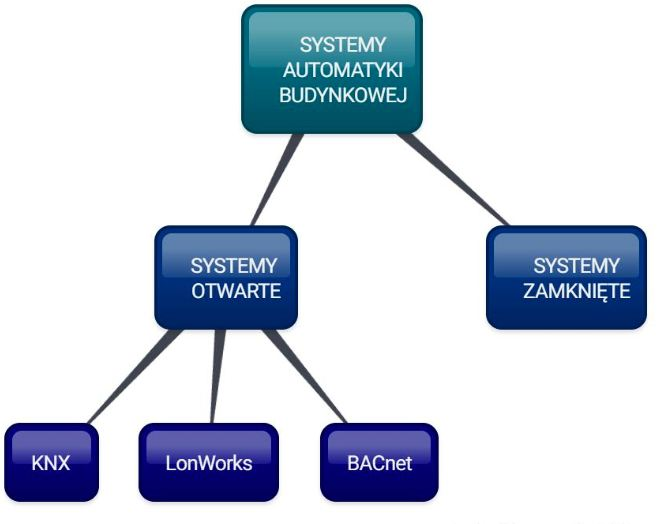
\includegraphics[scale=0.5]{files/systemy}
	\caption[Podział systemów]{Podział systemów automatyki budynkowej ze względu na kompatybilność urządzeń}
\end{figure}

\newpage
\chapter{Projekt i realizacja sterownika}
\ods W rozdziale tym przedstawiono proces tworzenia sterownika, parametry użytych komponentów, istotę sterowania, część programu źródłowego oraz schematy wykonanych obwodów. Konstruktor zada sobie również pytanie:\\
\textbf{Czy, sterownik ten, można zaprogramować do pracy w systemie KNX, by mógł się on kontaktować z urządzeniami innych producentów ?}

\newpage
\subsection{Transceiver NCN5120}
Układ NCN5120 to transceiver KNX, firmy ON Semiconductor,\\ o specyfikacji:

\begin{table}[h]
	\centering
	\begin{tabular}{l}
		$\bullet$transmisja z prędkością 9,6 kbps,\\
		$\bullet$regulacja poboru prądu z magistrali KNX ,\\
		$\bullet$dwa stabilizatory wbudowane:\\
		\ods $\cdot$stabilizator 3,3 [V],\\
		\ods $\cdot$stabilizator regulowany 3,3 - 21 [V],\\
		$\bullet$możliwe przejście w tryb uśpienia,\\
		$\bullet$wybór interfejsu komunikacyjnego między NCN a hostem:\\
		\ods $\cdot$UART : 8,9b/19200 bps, 8,9b/38400 bps,\\
		\ods $\cdot$SPI :  8b/125 kbps, 8b/500 kbps,\\
		$\bullet$taktowanie 16[MHz],\\
		$\bullet$umożliwia taktowanie urządzeń zewnętrznych 8/16[MHz],\\
		$\bullet$możliwa kontrola parzystości między hostem a NCN (Tylko dla UART),\\
		$\bullet$dostępny w jednej obudowie QFN40.\\
	\end{tabular}
\end{table}


\chapter{Podsumowanie}
\ods Z

% NEW PAGE
\newpage
\ods Z

% NEW PAGE
\newpage
\listoffigures

% NEW PAGE
\newpage
\listoftables

% NEW PAGE
\newpage
\begin{thebibliography}{99}
\bibitem{knx-basic} \textit{,,KNX Basic''} : www.knx.org (dostęp 10.01.2017)
\bibitem{knx-ar2} \textit{,,KNX System Specifications - Architecture''} : 06.2004 : www.sti.uniurb.it (dostęp 10.01.2017)
\bibitem{knx-protocol} \textit{,,Serial Data Transmission and KNX Protocol''} : www.knx.org (dostęp 10.01.2017)
\bibitem{knx-control} \textit{,,KNX System arguments''} : www.knx.org (dostęp 10.01.2017)
\bibitem{knx-guide} \textit{,,KNX Project Design Guidelines''} : www.knx.org (dostęp 10.01.2017)
\bibitem{knx-korea} D. K. Park, W. S. Lee, S. H. Hong, Luca Domenico Luigi Mazzon \textit{,,Development of a KNX/EIB-based Lighting Control System ''} :  Hanyang University at Ansan, Korea www.web.ics.purdue.edu (dostęp 10.01.2017)
\bibitem{petykiewicz} Paweł Petykiewicz \textit{,,Technika Systemowa Budynku Instabus EIB - Podstawy Projektowania''} : Warszawa, 1999 : www.we.pb.edu.pl (dostęp 10.01.2017)
\bibitem{ozadowicz} Mgr inż. Andrzej Ożadowicz \textit{,,Analiza porównawcza
dwóch systemów sterowania inteligentnym budynkiem –
systemu europejskiego EIB/KNX oraz standardu amerykańskiego
na bazie technologii LonWorks''} Rozprawa Doktorska, Kraków, 2006 : www.winntbg.bg.agh.edu.pl (dostęp 10.01.2017)
\bibitem{NCN} \textit{,,NCN5120 - Transceiver for KNX Twisted Pair Networks''} : Październik, 2015 : www.onsemi.com (dostęp 10.01.2017)
\bibitem{nucleo} \textit{,,STM32 Nucleo-64 board''} : Listopad, 2016 : www.st.com (dostęp 10.01.2017)
\bibitem{stm-rm} \textit{,,RM0351 Reference manual - STM32L4x6 advanced ARM®-based 32-bit MCUs''} : Czerwiec, 2016 : www.st.com (dostęp 10.01.2017)
\bibitem{hal} \textit{,,UM1884 - Description of STM32L4 HAL and Low-layer drivers''} : luty, 2016 : www.st.com (dostęp 10.01.2017)

\end{thebibliography}



\end{document}
